\section{Описание подхода}

TalkNet разбивает генерацию мэл-спектрограммы из текста на два отдельных модуля. Первый модуль, предсказатель длительности, выравнивает входные графемы по времени относительно звуковой дорожки (или мэл-спектрограммы, что то же самое так так длина мэл-спектрограммы линейно зависит от длины аудио). Второй модуль, генератор мэл-спектрограмм, производит генерацию из выровненных по времени входных символов (Рисунок~\ref{fig:arch}). Были использованы конволюционные модели прямого вывода (feed-forward) для обоих модулей, поэтому как обучение, так и вывод не являются авторегрессионными. Это позволяет гораздо быстрее обучаться и делать вывод по сравнению с авторегрессионными подходами. Для обучения предсказателя, истинные длительности графем извлекались из выхода CTC для предварительно обученной модели распознавания речи (Automatic-Speech-Recognition, ASR).

Таким образом, вводя дополнительный шаг на пути к получению мэл-спектро\-грамм, появляется возможность явным образом контролировать манеру произношения (просодию). Длительности букв можно изменить вручную, указав где нужно сделать паузу, а где наоборот проговорить быстро. Обе части могут обучаться независимо и параллельно, поэтому такой переход от end-to-end архитектуре к нескольким шагам оправдан с точки зрения времени.

\subsection{Извлечение истинных длительностей графем}

Центральная идея TalkNet заключается в использовании модели ASR на основе Connectionist Temporal Classification (CTC) функции ошибки для извлечения выравниваний графем. CTC присваивает вероятность каждому из символов алфавита и использует вспомогательный пустой символ $\sim$. Первым шагом схлопываются соседние повторявшиеся символы в выводе, подсчитывая таким образом длительность каждого символа. Пустой символ выступает как промежуточное состояние между двумя соседними графемами, и его длительность соответствует длительности перехода от одного символа к другому. Для каждого временного шага выбирается наиболее вероятный символ из выходных данных CTC (Рисунок~\ref{fig:ctc}).

\begin{figure}[!ht]
\centering
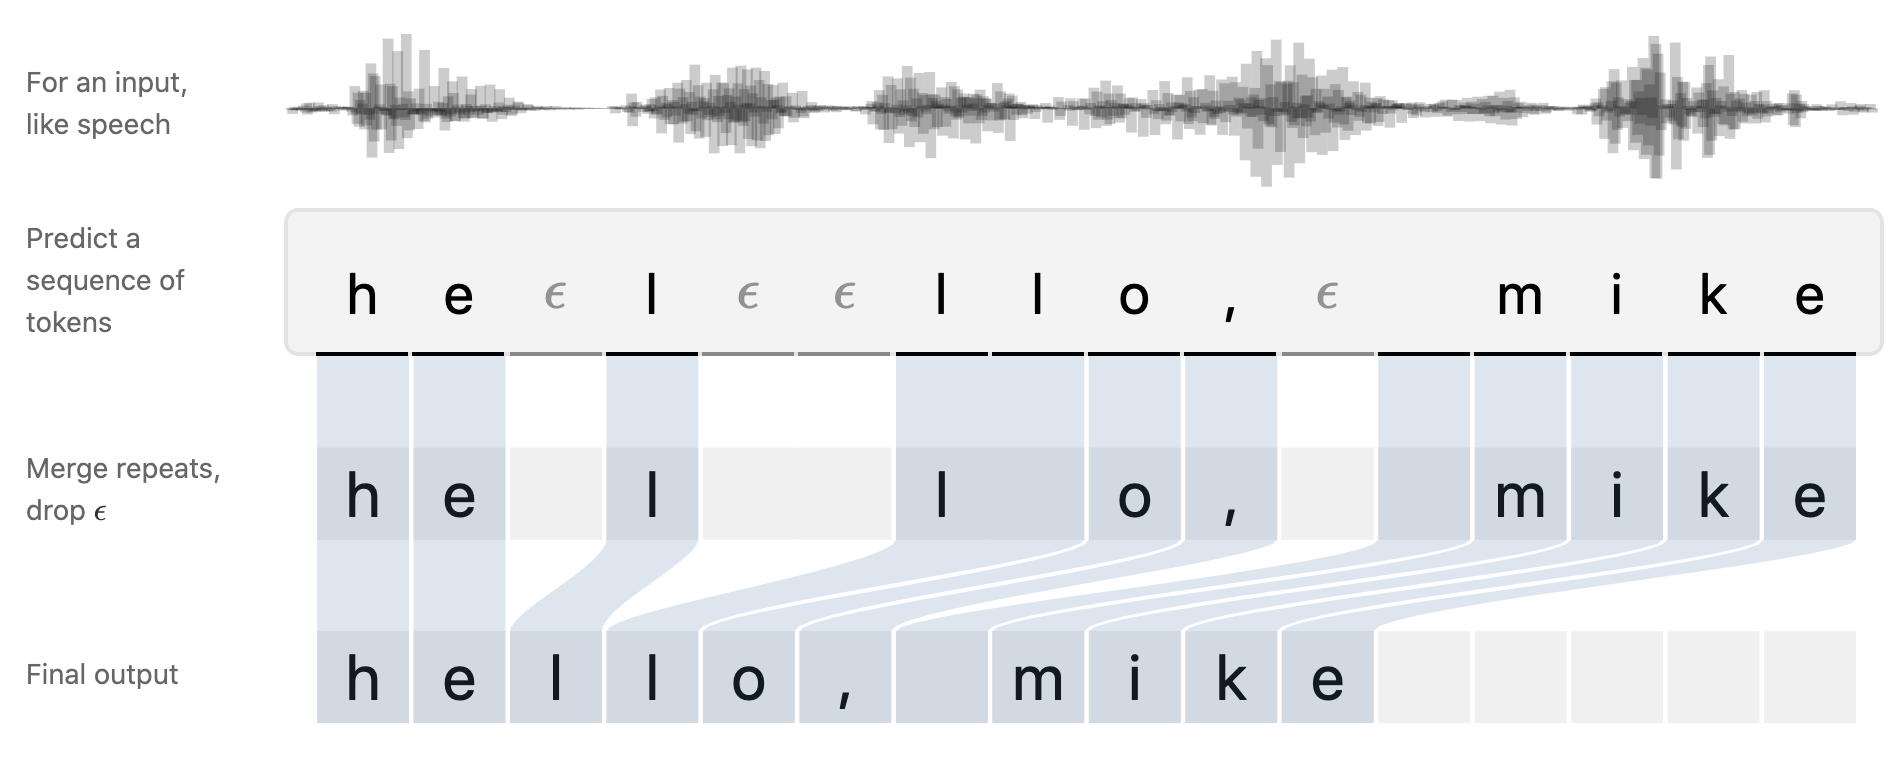
\includegraphics[width=1.0\textwidth]{images/snippets/ctc.png}
\caption{Пример работы CTC алгоритма~\cite{hannun2017sequence}. Соседние буквы схлопываются, а $\epsilon$ ($\sim$ в нашей нотации) служит разделительным вспомогательным символом.}
\label{fig:ctc}
\end{figure}

CTC -- это функция ошибки, используемая для этапа обучения. Поэтому, выход CTC часто бывает неточен. Однако, задача ASR решена намного лучше TTS, поэтому ошибка все еще намного меньше. Выход CTC выравнивается с истинным отрывком текста для того чтобы максимально устранить влияние ошибки. Была использована функция \textit{pairwise2} из пакета Biopython~\cite{biopython} (пакет для использования в биоинформатике для языка Python), которая выравнивает два строковых представления побуквенно, используя наименьшее количество операции добавления и удаления символов. Затем удаляются все неправильные символы в выводе CTC, а их длительность добавляется к ближайшему пустому, а также добавляются недостающие символы с длительность $0$. Затем, все символы с предсказанной длительностью 0 получают длительность 1, вычитая 1 из почти самого большого соседнего $\sim$, чтобы сумма всех длительностей графемы была равна длине мэл-спектрограммы (Рисунок~\ref{fig:alignment}).

\begin{figure}[!ht]
\centering
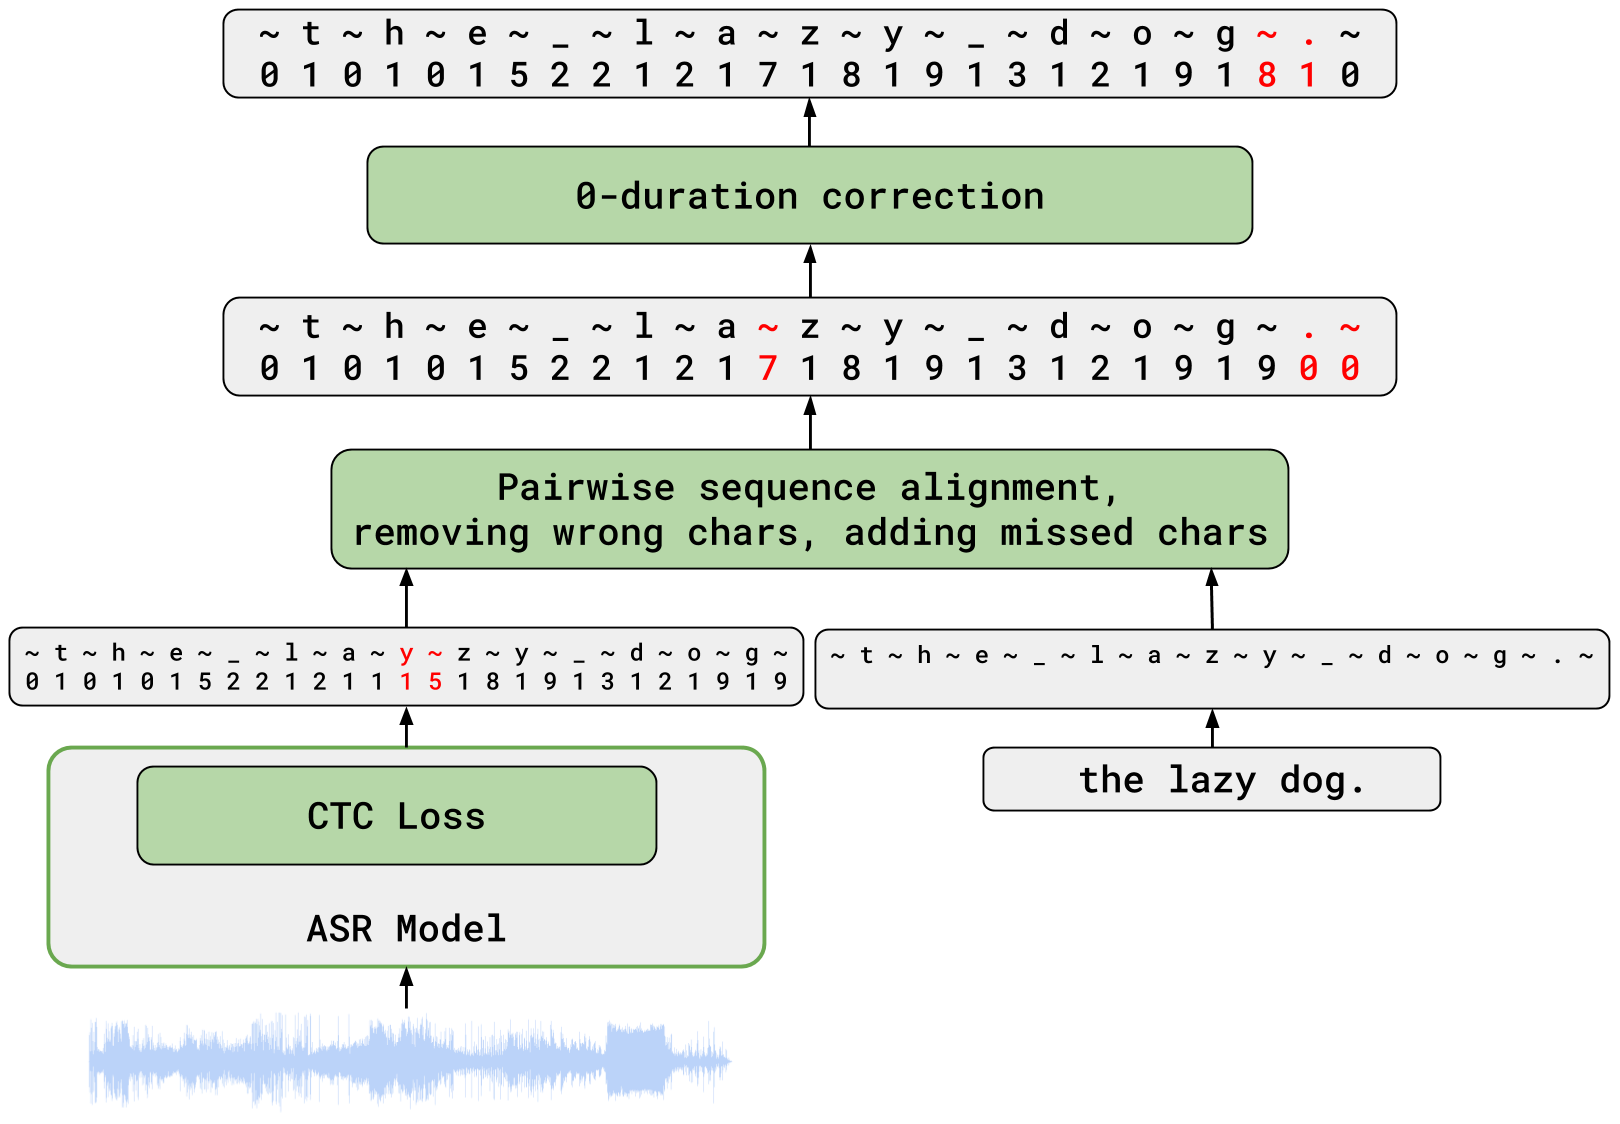
\includegraphics[width=1.0\textwidth]{images/alignment.png}
\caption{Извлечение длительности графемы из вывода CTC. $\sim$ используется для обозначения пустого символа в CTC.}
\label{fig:alignment}
\end{figure}

В качестве модели с CTC выводом для задачи распознавания текста (ASR) используется QuartzNet~\cite{quartznet}. QuartzNet (Рисунок~\ref{fig:qn}) -- это полностью коволюционная нейронная архитектура, основными достоинствами которой являются:
\begin{itemize}
    \item Низкое количество параметров (около 18 миллионов), которое было достигнуто за счет использования depthwise separable~\cite{kaiser2017depthwise} конволюций, являющихся математическим приближение обычных конволюций (Рисунок~\ref{fig:dws-conv}).
    \item Простая неавторегрессионная архитектура с базовыми операциями из глубокого обучения (конволюции, нелинейности, батч-нормализация и дропаут), позволяющяя значительно ускорить процесс обучения и вывода (inference).
    \item CTC функция в качестве функции ошибки в декодере, которая не содержит дополнительных параметров и обеспечивает быстрый вывод.
\end{itemize}

\begin{figure}[!ht]
\centering
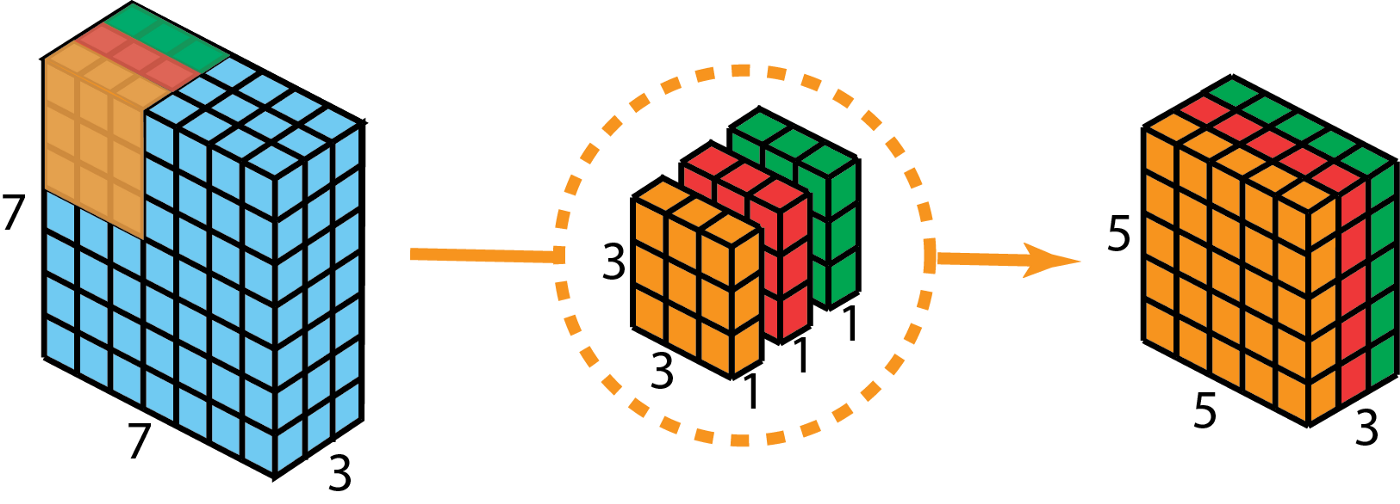
\includegraphics[width=1.0\textwidth]{images/snippets/dws-conv-1.png}
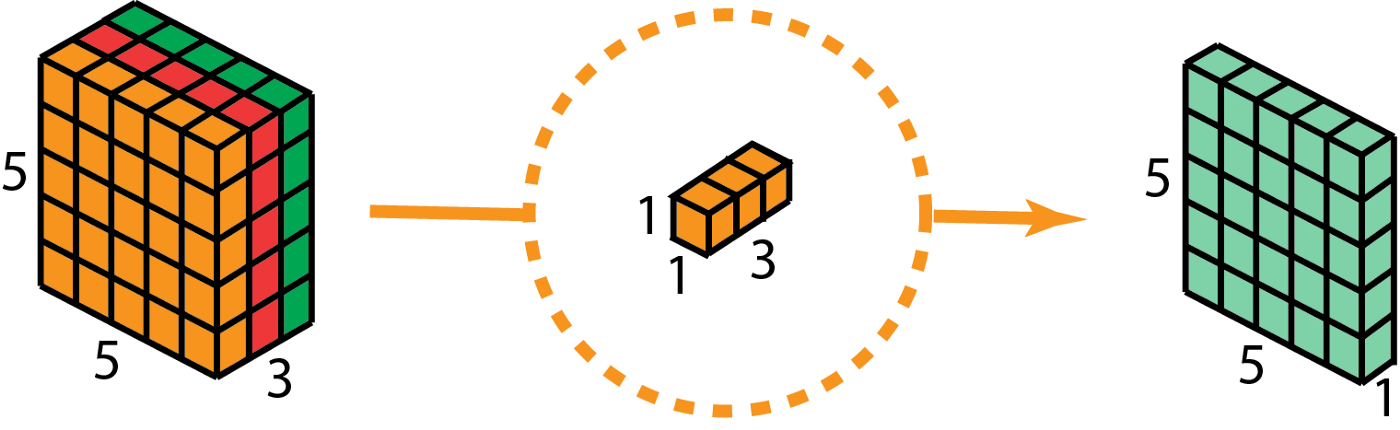
\includegraphics[width=1.0\textwidth]{images/snippets/dws-conv-2.png}
\caption{Depthwise separable конволюции. Применяется в два этапа: на первом используется 1d конволюции по времени, на втором применяются $1x1$ pointwise свертки. Два шага работают сообща и действуют как аппроксимация обычных сверток к квадратичными ядрами. В TalkNet такие свертки реализованы напрямую, через две последовательные конволюции.}
\label{fig:dws-conv}
\end{figure}

\begin{figure}[!ht]
\centering
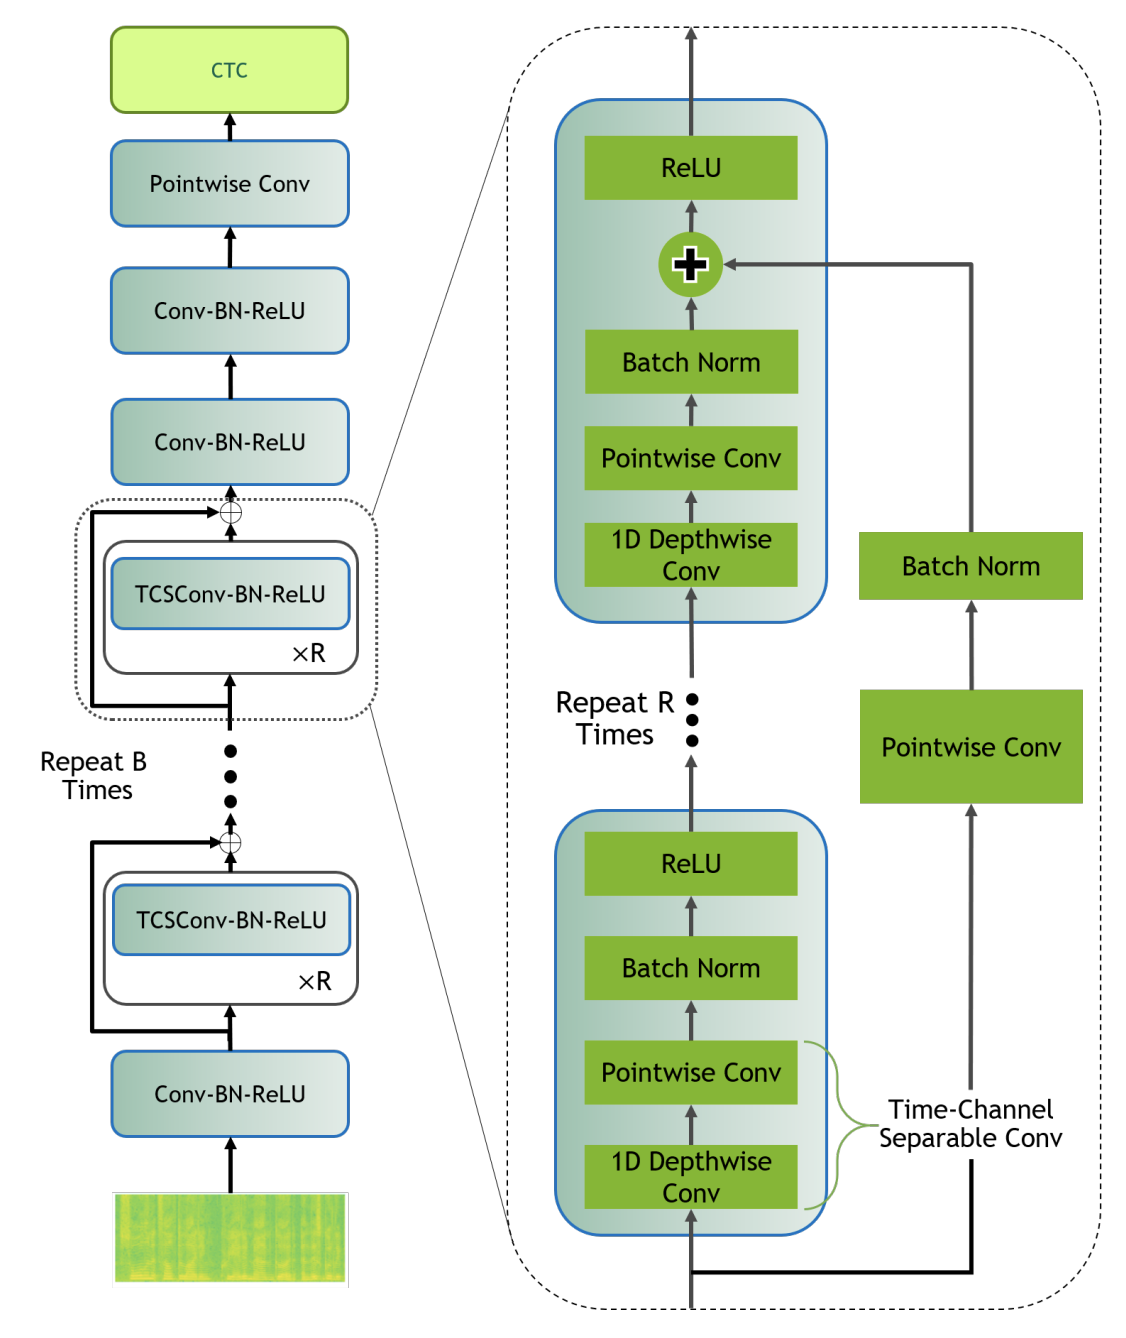
\includegraphics[width=0.8\textwidth]{images/qn.png}
\caption{Оригинальная архитектура QuartzNet 15x5}
\label{fig:qn}
\end{figure}

Для получения истинных длительностей графем была использована архитектура QuartzNet 15x5 (15 блоков по 5 повторений). Выход такой модели по длине в 2 раза меньше входной мэл-спектрограммы. Причина -- в самой первой конволюции выставлен параметр $\texttt{stride}=2$ (Рисунок~\ref{fig:stride-2}). QuartzNet использует удвоение шага в самом начале, так как для любого примера длина выходного текста как минимум в два раза меньше длины мэл-спектрограммы, поэтому такой трюк позволяет сократить количество вычислений вдвое. Однако, это так же уменьшает длительность каждого символа в выходе CTC. Чтобы сравнять сумму длительностей с длиной мэла, QuartzNet претерпела изменения, устанавливая $\texttt{stride}=1$ для первого слоя. Заметим так же что это не убирает возможность воспользоваться предобученной моделью, загрузив веса перед обучением для дообучения (fine-tuning) -- размеры, форма и количество ядер (kernels) конволюций остается неизменным. Соответственно, не изменяются и размеры матриц и векторов с весами.

\begin{figure}[!ht]
\centering
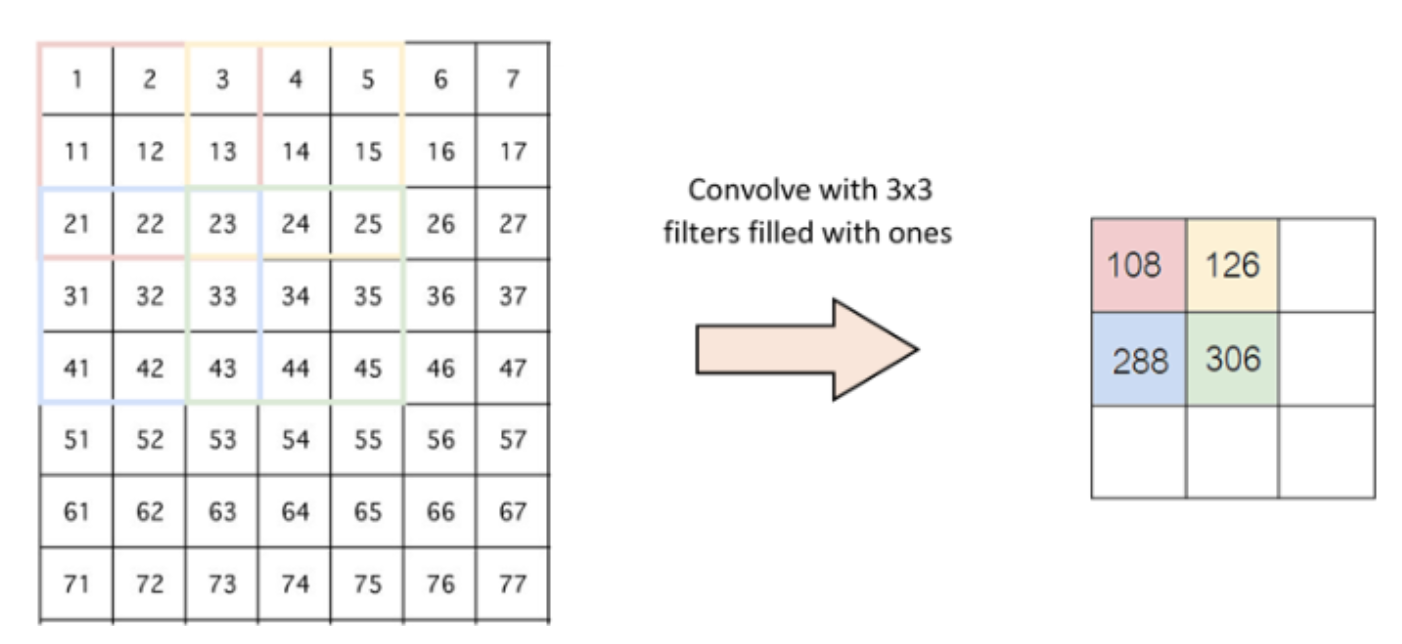
\includegraphics[width=0.8\textwidth]{images/snippets/stride-2.png}
\caption{Пример работы конволюций с удвоенным шагом}
\label{fig:stride-2}
\end{figure}

QuartzNet 15x5 дообучался на данных из датасета LibriTTS~\cite{libritts}. LibriTTS это набор данных из того же источника, что и LibriSpeech, на котором успешно обучался оригинальный QuartzNet. Однако, LibriTTS использует другую обработку данных, которая более подходит для задач генерации речи, нежели распознавания речи. В частности, LibriTTS обрезает отрывки аудио по большим паузам, оставляет всю пунктуацию нетронутой (для экспрессивности речи), а также разворачиваем некоторые числа и буквенные сокращения. Для токенизации входного текста (разбиения на символы) была оставлена вся пунктуацию, давая возможность CTC самому назначит длительность каждому символу. При дообучении QuartzNet на LibriTTS достигалась побуквенная ошибка (Char-Error-Rate, CER) порядка $4.51\%$ на части dev-clean и порядка $3.54\%$ на тестовой части LJSpeech~\cite{ljspeech}. Выравнивание, полученное из CTC, используется для обучения предиктора длительности графемы.

Таким образом, вместо того чтобы использовать другую преодобученную TTS модель в качестве учителя для получения длительностей графем, как это делалось в модели FastSpeech~\cite{fastspeech}, в рамках данной работы представлен метод в котором используется ASR модель. Ошибка, получаемая в CTC гораздо меньше ошибки при генерации речи, поэтому такой способ позволяет снять жесткое ограничение на качество, задаваемой моделью учителя.

\subsection{Предсказатель длительностей графем}

Первая часть TalkNet'а служит для предсказания длины мэл-спектрограммы с помощью соответствия каждому входному символу (включая пунктуацию) количество единиц времени, требуемых для их вывода. Первым шагом предиктор длительностей вставляет пустой символ $\sim$ между каждыми двумя соседними символами. Затем он предсказывает длительность для каждого входного символа с помощью конволюционной нейронной архитектуры. Далее, производится операция расширения (expansion) входных символов в соответствии с предсказанной длительностью (Рисунок~\ref{fig:durs}).

\begin{figure}[!ht]
\centering
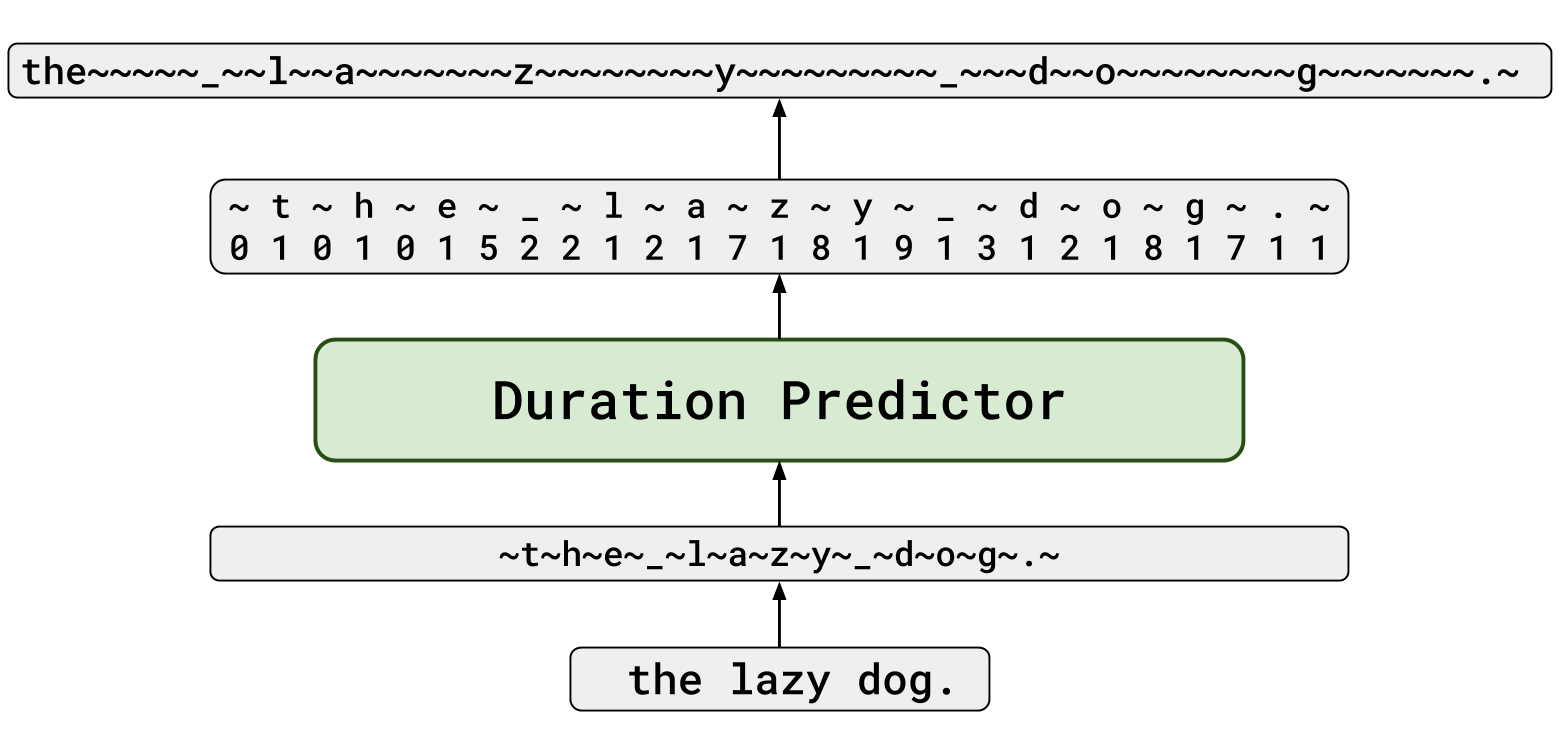
\includegraphics[width=1.0\linewidth]{images/durs.png}
\caption{Процесс предсказания длительностей графем}
\label{fig:durs}
\end{figure}

Модель предиктора длительностей представляет собой конволюционную нейронную сеть, основанную на архитектуре модели для распознавания речи QuartzNet~\cite{quartznet}. Модель имеет $5$ больших блоков с 5 повторениями на блок. Подблок состоит из depthwise separable~\ref{fig:dws-conv} конволюции, батч нормализации, нелинейности ReLU и дропаута (Рисунок~\ref{fig:qn-block}). Помимо этого, применяются два дополнительных слоя: обучаемая векторизация токенов графем и $1x1$ слой перед передачей в функцию потери (Таблица~\ref{tab:durs-model}). Размерность последнего слоя зависит от типа функции потерь: для $L_2$ это 1, для кросс-энтропии это $|\texttt{множество\_классов}|$.

\begin{figure}[!ht]
\centering
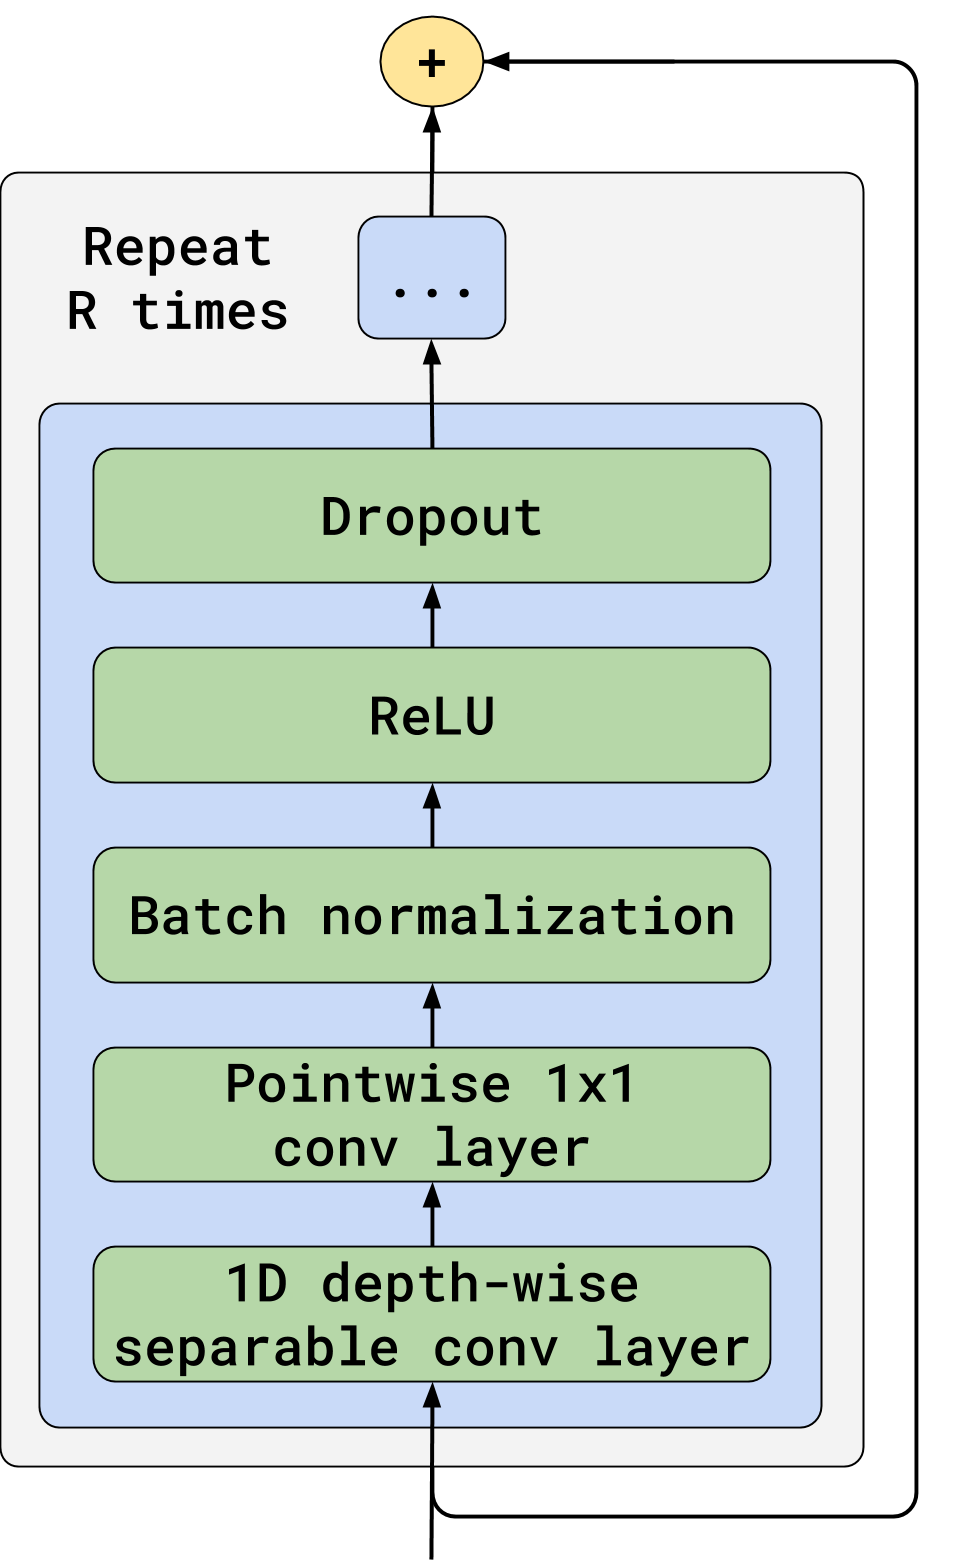
\includegraphics[width=0.6\linewidth]{images/qn-block.png}
\caption{Базовый блок QuartzNet. Как предиктор длительностей графем, так и генератор мэл-спектрограмм являются сверточными сетями с 1D time-channel свертками на основе QuartzNet~\cite{quartznet}.}
\label{fig:qn-block}
\end{figure}

Тренировка предиктора длительностей происходит при использовании $L_2$ функции ошибки с логарифмированием целевых значений аналогично~\cite{fastspeech}. Таким образом, больший вес при обучении присваивается символам с меньшими длительностями. В самом деле, разница между $15$ и $16$ не такая значительная как между $1$ и $2$. Была также испробована другая функция ошибки -- кросс-энтропийные критерий, где каждый класс соответствовал определенной длительности. При классификации, были выбраны $32$ самых частых класса (первые $32$ длительности -- от $0$ до $31$), а также добавлены редкие большие длительности с логарифмическим шагом после $32$, так как распределение длительности графемы имеет длинный хвост (Рисунок~\ref{fig:durs-dist}). Как можно видеть, кросс-энтропия имеет несколько более высокую поклассовую точность (Таблица~\ref{tab:dur-results}). Однако, в рамках данной работы будет использоваться $L2$, так как речь, сгенерированная с меньшим MSE для длительностей, получила несколько более высокий mean opinion score (MOS) в процессе валидации.

\begin{figure}[!ht]
\centering
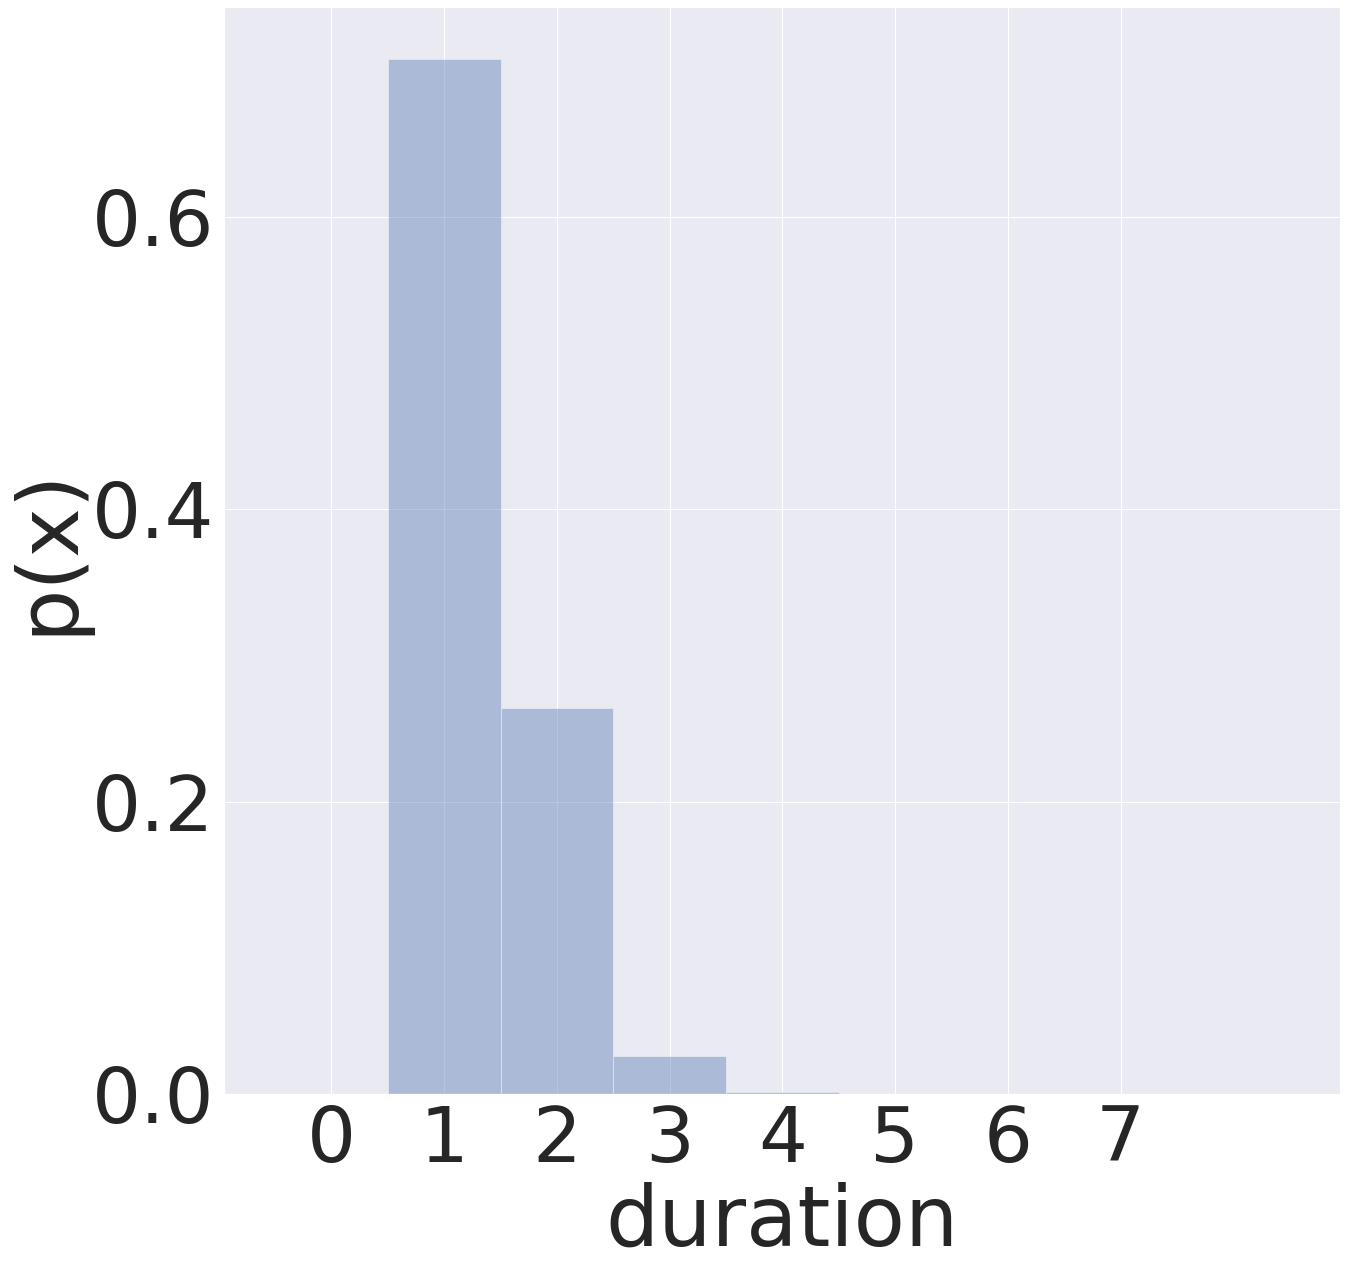
\includegraphics[width=.48\linewidth]{images/durs-dist.png}
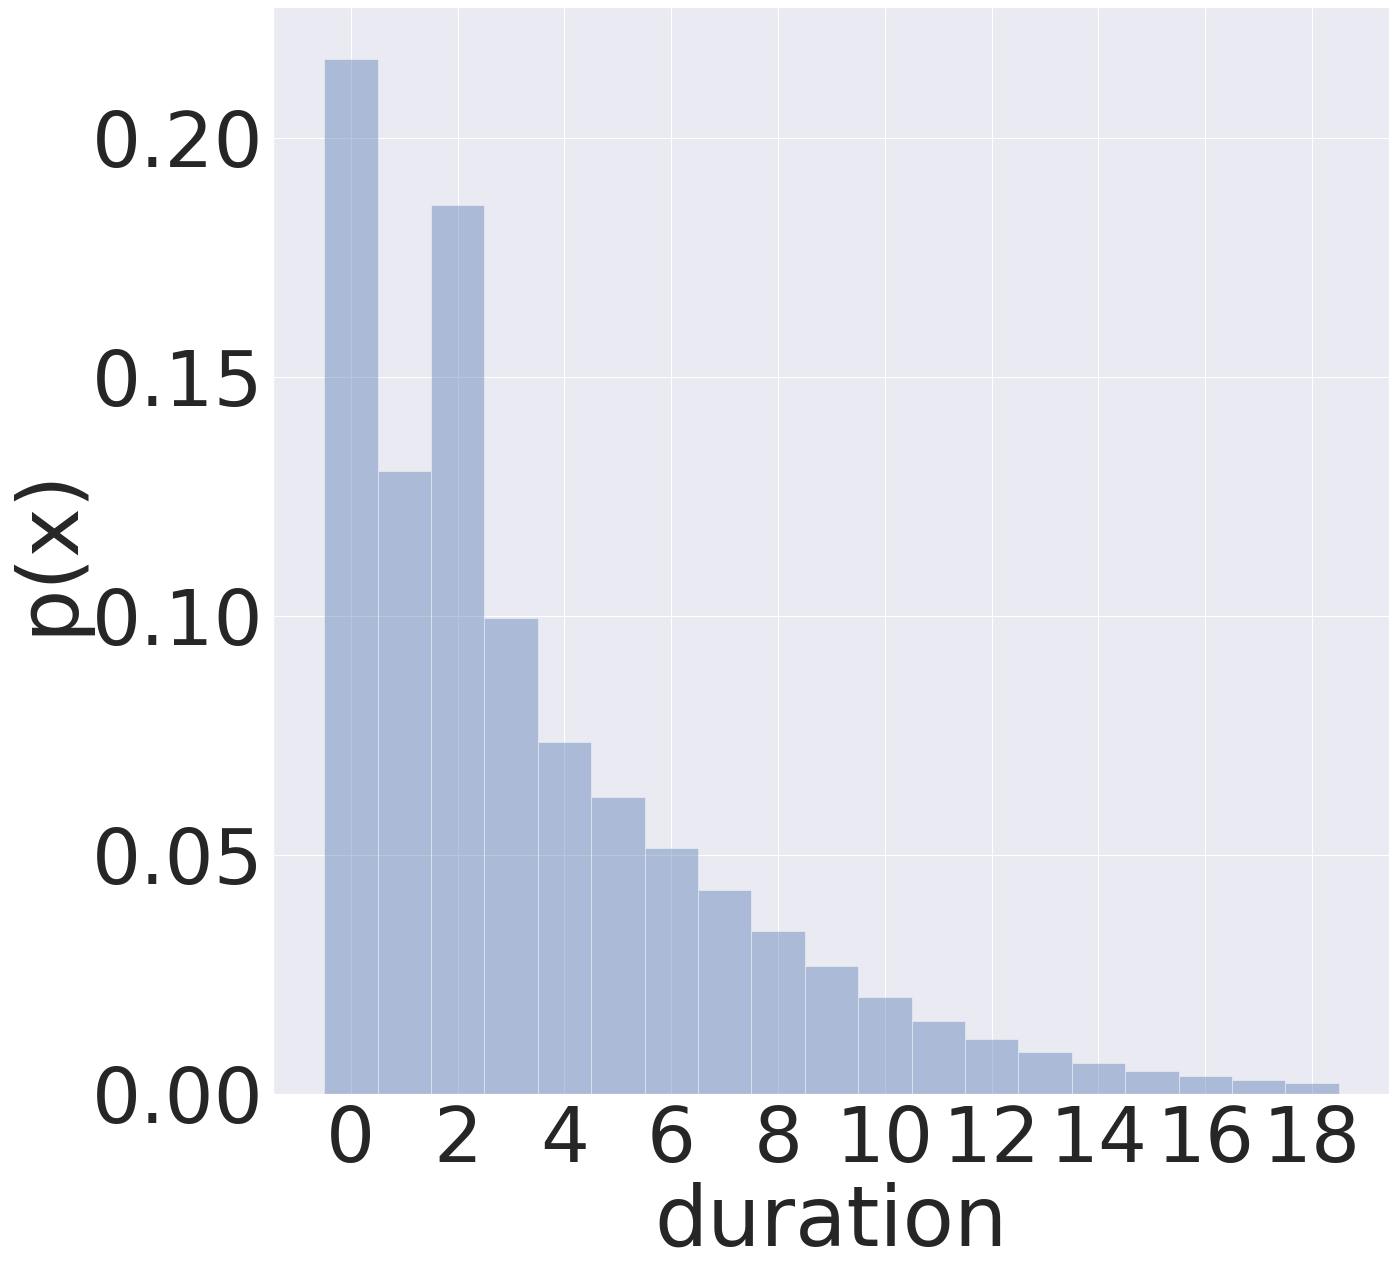
\includegraphics[width=.48\linewidth]{images/blanks-dist.png}
\caption{Распределение длительностей исходных символов (слева) и символов перехода (справа) на основе вывода CTC для набора данных LJSpeech. Максимальная длительность для символов составляет $7$, а для $\sim$ - $493$.}
\label{fig:durs-dist}
\end{figure}

\begin{table}[!ht]
\centering
\scalebox{1.2}{
\begin{tabular}{c c c c c} 
\toprule
\textbf{Block} &
\textbf{\thead{\# Sub\\Blocks}} &
\textbf{\thead{\# Output\\Channels}} &
\textbf{Kernel Size} &
\textbf{Dropout} \\
\midrule
Embed & 1 & 64  & 1 & 0.0  \\
Conv1 & 3 & 256 & 3 & 0.1  \\
$B_1$ & 5 & 256 & 5 & 0.1  \\
$B_2$ & 5 & 256 & 7 & 0.1  \\
$B_3$ & 5 & 256 & 9 & 0.1  \\
$B_4$ & 5 & 256 & 11 & 0.1 \\
$B_5$ & 5 & 256 & 13 & 0.1 \\
Conv2 & 1 & 512 & 1 & 0.1  \\
Conv3 & 1 & $32$ & 1 & 0.0 \\
\midrule
\textbf{Params, M} & & & & \textbf{2.3} \\
\bottomrule
\end{tabular}
}
\caption{Предиктор длительностей графем основан архитектуре QuartzNet 5х5. Residual соединения и увеличивающиеся размеры сверток позволяют эффективно выучивать различнные паттерны и комбинировать их на поздних слоях.}
\label{tab:durs-model}
\end{table}

\begin{table}[!ht]
\centering
\scalebox{1.2}{
\begin{tabular}{c c c c c c c} 
\toprule
\textbf{Method} &
\textbf{MSE} &
\textbf{Accuracy, $\%$} &
$\mathbf{|P - T| \leq 1}$ &
$\mathbf{|P - T| \leq 3}$\\
\midrule
$L_2$ & 7.81 & 67.69 & 91.90 & 97.17 \\
XE & 10.46 & 69.42 & 92.90 & 97.40 \\
\bottomrule
\end{tabular}
}
\caption{Результаты предиктора длительностей на тестовой части LJSpeech. $P$ - предсказание, $T$ - целевое значение.}
\label{tab:durs-results}
\end{table}

\subsection{Генератор мэл-спектрограмм}

Второй модуль производит генерацию мэл-спектрограммы из развернутого текста. Генератор представляет собой сверточную сеть, также основанную на архитектуре QuartzNet. Он имеет 9 блоков с 5 подблоками (Таблица\ref{tab:mels-model}). Как можно видеть, размер ядер конволюций увеличивается от слоя к слою с 5 до 25. Это, вкупе с residual ребрами вычислительного графа, позволяют модели выучить паттерны разного размера для применения на входной последовательности и объединить их на поздних слоях для предсказания мэл-спектрограммы. На входе также действует слой с эмбеддингом входной последовательности и дополнительная 3x3 конволюция. На выходе стоит 1x1 конволюция с размером выхода в 80 -- длиной одного мэл вектора. Генератор мэл-спектрограмм был обучен с функций ошибки -- усредненной среднеквадратичной потерей (Mean-Square-Error, MSE) между элементами матриц.

Пустой $\sim$ символ дополняет алфавит исходной входной последовательности. Но вместо того, чтобы выделять для него отдельный вектор в таблице embeddings первого слоя генератора мэл-спектрограмм, он заменяется на линейную комбинацию эмбеддингов для соседним графем. Более точно, если пустой символ $\sim$ расположен между символами $a$ и $b$, его длительность равна $d$, то эмбеддинг $E$ для $\sim$ расположенного на расстоянии $t$ слева от $a$ будет равен $E (\sim, t) = \dfrac{d+1-t}{d+1} \cdot E(a) + \dfrac{t}{d+1} \cdot E (b)$. Это более точно соответствует смысловой нагрузке пустого символа, являющегося промежуточным символам в переходе от $a$ к $b$ и помогает модели быстрее обучаться.

\begin{table}[!ht]
\centering
\scalebox{1.2}{
\begin{tabular}{c c c c c} 
 \toprule
  \textbf{Block} &
  \textbf{\thead{\# Sub\\Blocks}} &
  \textbf{\thead{\# Output\\Channels}} &
  \textbf{Kernel Size} &
  \textbf{Dropout} \\
 \midrule
Embed & 1 & 256 & 1 & 0.0 \\
Conv1 & 3 & 256 & 3 & 0.0 \\
$B_1$ & 5 & 256 & 5 & 0.0 \\
$B_2$ & 5 & 256 & 7 & 0.0 \\
$B_3$ & 5 & 256 & 9 & 0.0 \\
$B_4$ & 5 & 256 & 13 & 0.0 \\
$B_5$ & 5 & 256 & 15 & 0.0 \\
$B_6$ & 5 & 256 & 17 & 0.0 \\
$B_7$ & 5 & 512 & 21 & 0.0 \\
$B_8$ & 5 & 512 & 23 & 0.0 \\
$B_9$ & 5 & 512 & 25 & 0.0 \\
Conv2 & 1 & 1024 & 1 & 0.0 \\
Conv3 & 1 & 80 & 1 & 0.0 \\
\midrule
\textbf{Params, M} & & & & \textbf{8.5} \\
\bottomrule
\end{tabular}
}
\caption{Параметры генератора мэл-спектрограмм с архитектурой, основанной на QuartzNet 9x5}
\label{tab:mels-model}
\end{table}

Глубина нейронной сети в 45 слоев (9 блоков по 5 подблоков) позволяет получить receptive field на последних слоях, накрывающий всю входную последовательность. Однако, он имеет неравномерную силу действия в зависимости от удаленности по времени. Это имеет простую интерпретацию: чем дальше от графемы (буквы) находиться другая графема, тем меньше она влияет на правильность произношения.

В общем и целом, представленная архитектура спроектирована таким образом, чтобы максимально устранить узкие места с точки зрения скорости и эффективности реализации на графических ускорителях. Отсутствие операций с механизмом внимания, широко использующимся в других подходов, позволяет получить максимальный эффект в рамках модели многопоточности GPU. Неавторегрессионность обоих шагов, а также явное предсказание длительностей, позволяет получить быструю устойчивую модель, сохраняя при этом возможность сохранить качество.